\documentclass[tikz,dvisvgm,border=1pt]{standalone}
% Shared preamble for the attribution infographics (iN-*.tex).
% tools/tikz-build.sh compiles each source with \variant set to wide or narrow.
\usepackage[T1]{fontenc}
\usepackage[default,semibold]{sourcesanspro}
\usepackage[italic]{mathastext}
% Larger scripts than the TeX default, so subscripts stay legible at phone width.
\DeclareMathSizes{9}{9}{8}{7}
\DeclareMathSizes{10}{10}{9}{8}
\DeclareMathSizes{11}{11}{9}{8}
\DeclareMathSizes{11.5}{11.5}{9.5}{8}
\usetikzlibrary{arrows.meta,positioning,calc,fit,backgrounds,decorations.pathreplacing,patterns}

\ifdefined\variant\else\def\variant{wide}\fi
\newif\ifnarrow
\def\narrowname{narrow}
\ifx\variant\narrowname\narrowtrue\fi
% The narrow variant is about 320pt wide and shown at about 350px, the wide one
% about 540pt wide and shown at up to 720px: the narrow one uses larger type.
\ifnarrow
  \def\basefont{\fontsize{11}{13}\selectfont}\def\smallfont{\fontsize{10}{12}\selectfont}
  \def\titlefont{\fontsize{11.5}{13.5}\selectfont\bfseries}
\else
  \def\basefont{\fontsize{10}{12}\selectfont}\def\smallfont{\fontsize{9}{11}\selectfont}
  \def\titlefont{\fontsize{11}{13}\selectfont\bfseries}
\fi

% Light-theme page tokens (web/src/styles/_variables.css, embeds.css), fixed:
% every infographic sits on its own light card, so it reads on both themes.
\definecolor{ink}{HTML}{262626}      % --text-color on white
\definecolor{muted}{HTML}{666666}    % --muted-color on white
\definecolor{rule}{HTML}{DCDCDC}     % --border-color, slightly stronger
\definecolor{surface}{HTML}{F5F5F5}  % --neutral-200
\definecolor{heading}{HTML}{904B20}  % h2 colour
\definecolor{info}{HTML}{187C9B}     % embeds --info-color
\definecolor{primary}{HTML}{C65928}  % embeds --primary-color
\definecolor{success}{HTML}{35814C}  % embeds --success-color
\definecolor{danger}{HTML}{BD3F50}   % f13 spread cost
\definecolor{residual}{HTML}{A77913} % f13 residual

\tikzset{
  every picture/.style={color=ink, line width=0.6pt, >={Stealth[length=5pt,width=4pt]},
    font=\basefont},
  small/.style={font=\smallfont},
  title/.style={font=\titlefont},
  box/.style={draw=rule, fill=white, rounded corners=4pt, align=center, inner sep=5pt},
  tag/.style={small, text=muted},
}

% No hyphenation in the narrow text columns of the diagrams.
\hyphenpenalty=10000 \exhyphenpenalty=10000

% Light card behind the whole drawing, below the background layer.
\pgfdeclarelayer{card}
\pgfsetlayers{card,background,main}
\newcommand\drawcard{%
  \begin{pgfonlayer}{card}
    \fill[white, draw=rule, rounded corners=8pt]
      ($(current bounding box.south west)+(-10pt,-10pt)$)
      rectangle ($(current bounding box.north east)+(10pt,10pt)$);
  \end{pgfonlayer}}

% Same hypothetical one-share fill as section 2.5; fees charged once.
\begin{document}
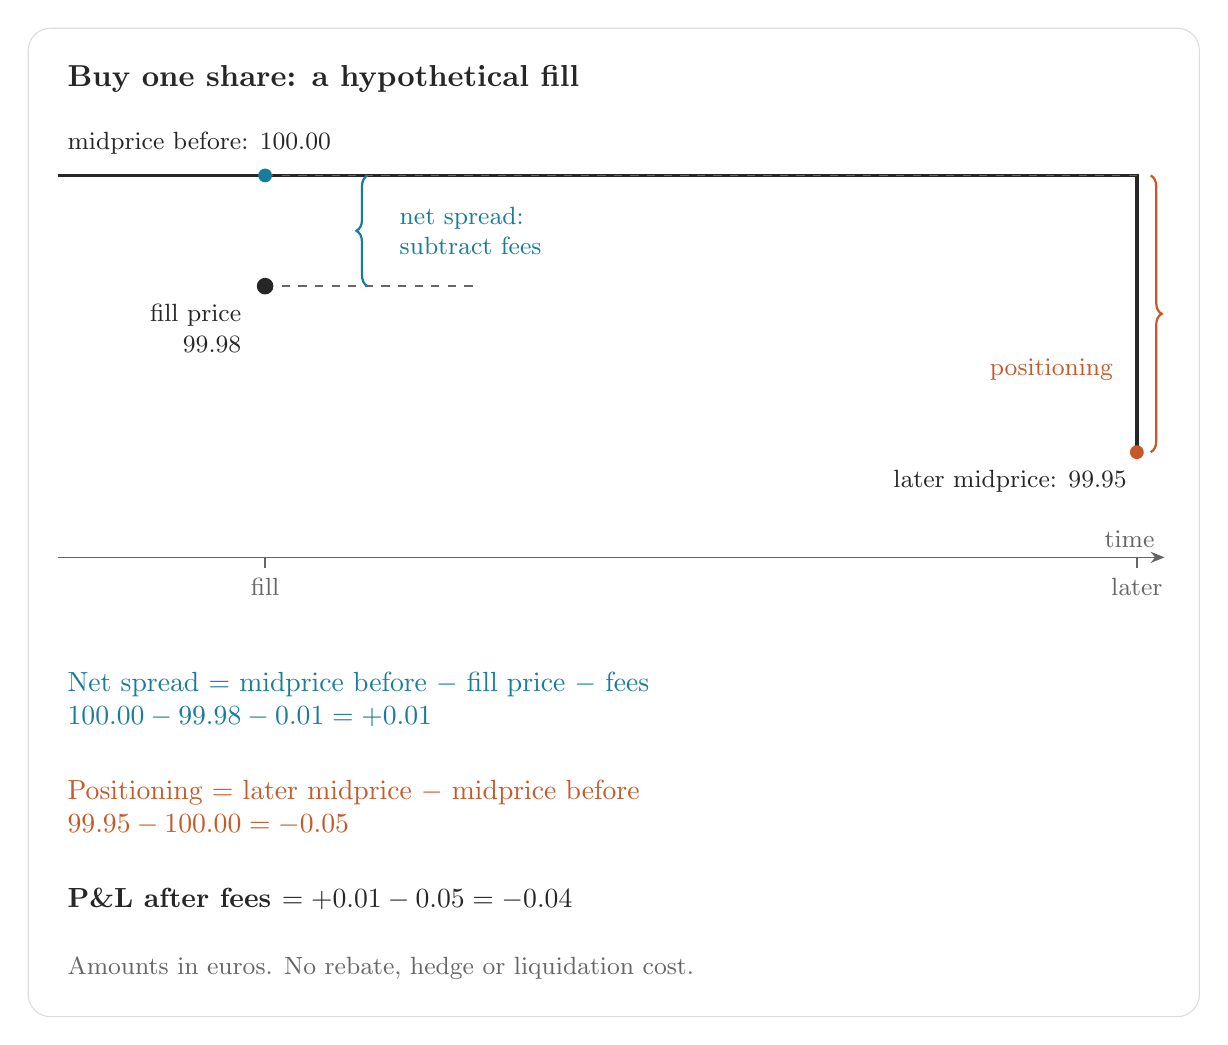
\begin{tikzpicture}
\ifnarrow
  \def\span{270pt}
\else
  \def\span{390pt}
\fi
\node[anchor=west,title] at (0,135pt) {Buy one share: a hypothetical fill};
% Midprice path and the execution price use one linear price scale.
\draw[ink,line width=1.2pt] (0,100pt) -- (\span,100pt) -- (\span,0);
\draw[muted,dashed] (75pt,100pt) -- (\span,100pt);
\draw[muted,dashed] (75pt,60pt) -- (150pt,60pt);
\fill[info] (75pt,100pt) circle (2.5pt);
\fill[ink] (75pt,60pt) circle (3pt);
\fill[primary] (\span,0) circle (2.5pt);
\node[anchor=south west,small] at (0,104pt) {midprice before: 100.00};
\node[anchor=north east,small,align=right] at (70pt,57pt) {fill price\\99.98};
\node[anchor=north east,small] at (\span,-3pt) {later midprice: 99.95};
% Brackets link price differences to their accounting components.
\draw[info,decorate,decoration={brace,amplitude=4pt},thick]
  (112pt,60pt) -- (112pt,100pt);
\node[anchor=west,small,text=info,align=left] at (120pt,80pt) {net spread:\\subtract fees};
\draw[primary,decorate,decoration={brace,amplitude=4pt},thick]
  (\span+5pt,100pt) -- (\span+5pt,0);
\node[anchor=east,small,text=primary] at (\span-5pt,30pt) {positioning};
\draw[->,muted] (0,-38pt) -- (\span+10pt,-38pt) node[above left,small] {time};
\draw[muted] (75pt,-38pt) -- ++(0,-4pt) node[below,small] {fill};
\draw[muted] (\span,-38pt) -- ++(0,-4pt) node[below,small] {later};
\node[anchor=north west,align=left,text=info] at (0,-76pt)
  {Net spread = midprice before $-$ fill price $-$ fees\\
   $100.00 - 99.98 - 0.01 = +0.01$};
\node[anchor=north west,align=left,text=primary] at (0,-115pt)
  {Positioning = later midprice $-$ midprice before\\
   $99.95 - 100.00 = -0.05$};
\node[anchor=north west,align=left,font=\basefont\bfseries] at (0,-154pt)
  {P\&L after fees $= +0.01 - 0.05 = -0.04$};
\node[anchor=north west,small,text=muted] at (0,-179pt)
  {Amounts in euros. No rebate, hedge or liquidation cost.};
\drawcard
\end{tikzpicture}
\end{document}
